\section*{Mòdul del parser}
Aquest mòdul actua com a pont entre l'entrada del programa i la representació intermèdia. La seva responsabilitat principal és instanciar el parser adequat, llegir el fitxer d'entrada, convertir l'\textit{AST} a elements normalitzats i retornar un resultat estructurat que pugui ser consumit per les anàlisis posteriors. A la implementació actual, la factoria \texttt{ParserFactory} decideix quin parser crear i, per a C\#, la classe \texttt{CSharpParser} usa Roslyn per obtenir el \texttt{SyntaxTree} i extreure la informació rellevant.

La figura~\ref{fig:parser_module} mostra el flux del mòdul: el fitxer entra al parser, el model del llenguatge es transforma mitjançant \texttt{CSharpElementMapper} i \texttt{ElementTranslator}, i finalment es retorna un \texttt{ParseResult} amb l'arrel del model i els diagnòstics generats durant la lectura. Aquest enfocament permet que la resta del sistema treballi sobre una estructura comuna i no depengui de la API específica de Roslyn.

\begin{figure}[H]
    \centering
    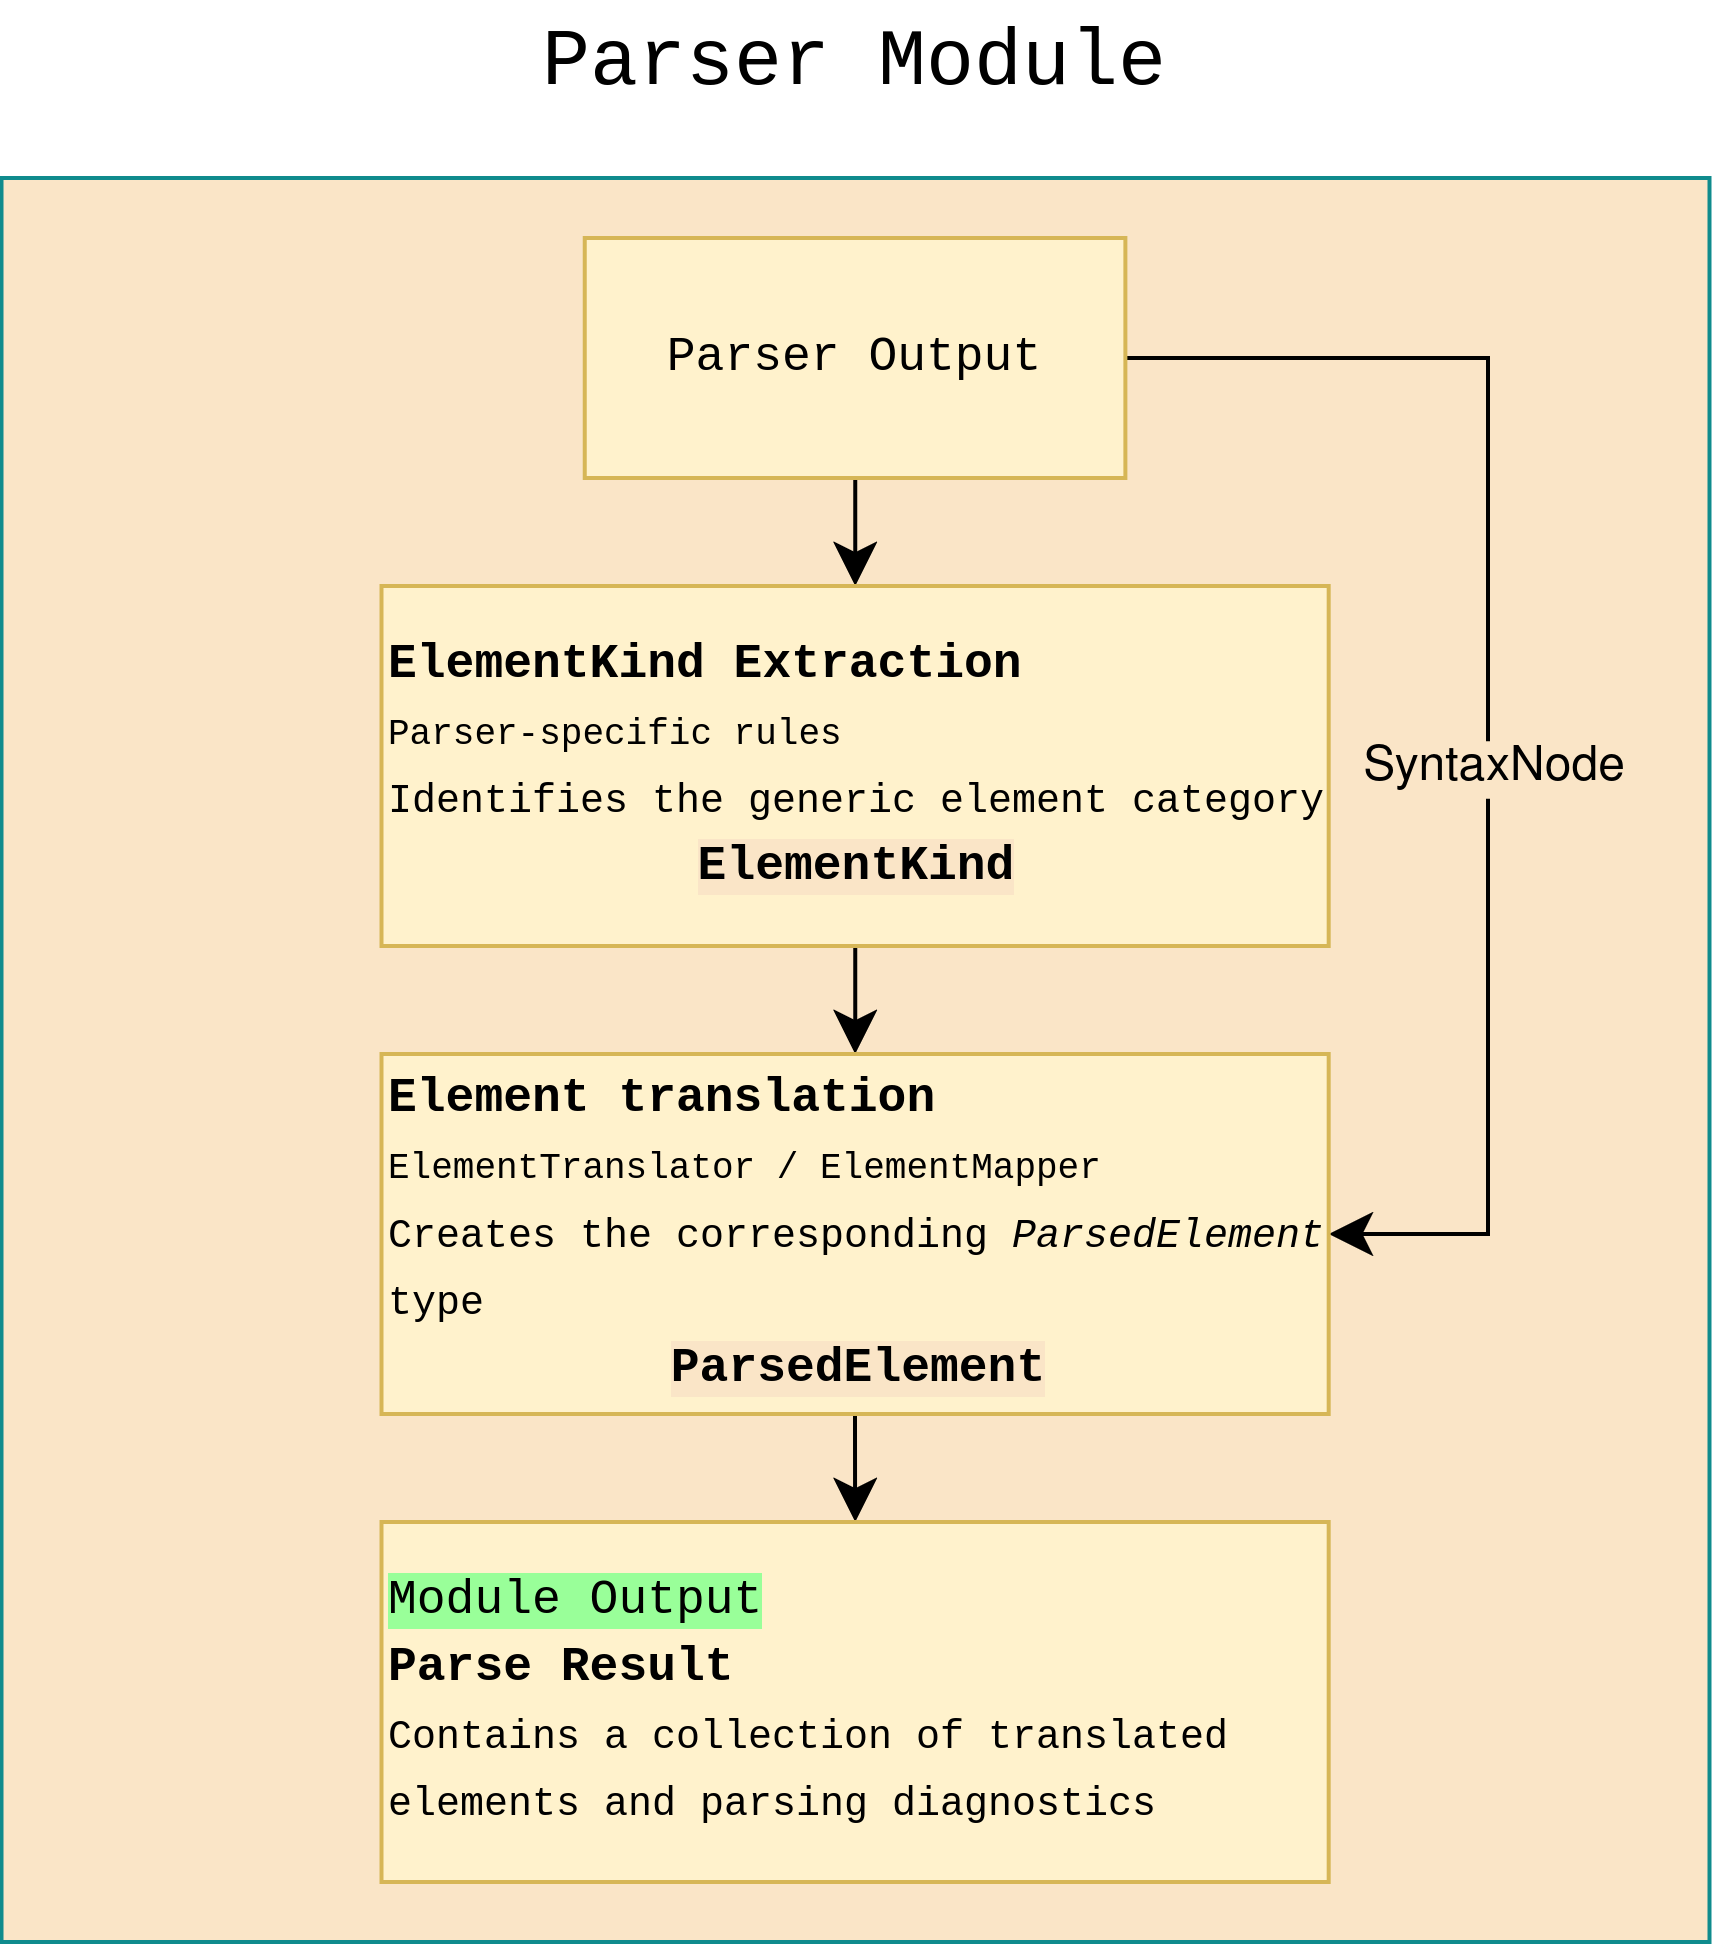
\includegraphics[width=0.8\textwidth]{../tfg/first_progress_report/figures/parser_module.png}
    \caption{Flux del mòdul del parser i adaptació del model de Roslyn a la representació comuna.}
    \label{fig:parser_module}
\end{figure}

El mòdul es pot desenvolupar de manera progressiva, començant per una versió inicial centrada en fitxers individuals i ampliant posteriorment la cobertura a projectes complets. Els objectius principals d'evolució són: \\
\\
\begin{tabular}{|c|c|}
    \hline
    \textbf{Versió inicial} & \textbf{Versió final} \\
    \hline
    Treball únicament amb fitxers individuals & Treball amb projectes complets \\ [0.3cm]
    \hline
    Detecció o especificació manual del llenguatge & Detecció automàtica del llenguatge \\ [0.3cm]
    \hline
    Instanciament manual del parser & Instanciament automàtic del parser \\ [0.3cm]
    \hline
\end{tabular}